\documentclass[11pt,a4paper]{article}
\usepackage[margin=2.5cm]{geometry}
\usepackage{amsmath,amssymb,amsthm,booktabs,array,graphicx,xcolor}
\usepackage[numbers,sort&compress]{natbib}
\usepackage{xr}
\externaldocument[M-]{manuscript}
\newcommand{\mref}[1]{\ref{M-#1}}
\newcommand{\meqref}[1]{(\ref{M-#1})}
\makeatletter\let\inputtbl\@@input\makeatother
\newlength{\tblwidth}\setlength{\tblwidth}{\linewidth}
\providecommand{\checkmark}{\ensuremath{\surd}}
\newcommand{\authorcheck}[1]{}
\newtheorem{remark}{Remark}[section]
\renewcommand{\theremark}{S\arabic{remark}}
\newenvironment{restated}[1]{\par\medskip\noindent\textbf{#1.}\ \itshape}{\par\medskip}
\renewcommand{\thetable}{S\arabic{table}}
\renewcommand{\thefigure}{S\arabic{figure}}
\renewcommand{\thesubsection}{S5.\arabic{subsection}}
% Shared by the LaTeX build (manuscript.tex) and the Word build (build_docx.py).
\newcommand{\negl}{\mathsf{negl}}
\newcommand{\PPT}{\mathrm{PPT}}
\newcommand{\Real}{\mathbf{Real}}
\newcommand{\Ideal}{\mathbf{Ideal}}
\newcommand{\Leak}{\mathcal{L}}
\newcommand{\Sim}{\mathcal{S}}
\newcommand{\Adv}{\mathcal{A}}
\newcommand{\cind}{\approx_c}
\newcommand{\Gen}{\mathsf{Gen}}
\newcommand{\Eval}{\mathsf{Eval}}
\newcommand{\Enc}{\mathsf{Enc}}
\newcommand{\Dec}{\mathsf{Dec}}
\newcommand{\advPRF}{\mathrm{Adv}^{\mathrm{prf}}}
\newcommand{\advDPF}{\mathrm{Adv}^{\mathrm{dpf}}}
\newcommand{\advCPA}{\mathrm{Adv}^{\mathrm{cpa}}}
\newcommand{\bplus}{\boxplus}
\newcommand{\bdot}{\boxdot}

\newcommand{\BuildIndex}{\mathsf{BuildIndex}}
\newcommand{\EncData}{\mathsf{EncData}}
\newcommand{\Compute}{\mathsf{Compute}}
\newcommand{\Token}{\mathsf{Token}}
\newcommand{\Setupp}{\mathsf{Setup}}
\newcommand{\bminus}{\boxminus}
\newcommand{\Search}{\mathsf{Search}}
\begin{document}
\begin{center}
{\Large\bfseries Supplementary Material}\\[4pt]
{\large Collusion-resilient, tamper-evident range analytics over homomorphically
encrypted Internet of Things data in multi-cloud storage}
\end{center}
\noindent Section, theorem, table and equation numbers without an ``S'' refer to
the main text. Tables and figures here are numbered S1, S2, \dots
\medskip
\section*{S1. Why a homomorphic layer at $t=n-1$: the full argument}
\addcontentsline{toc}{section}{S1. Why a homomorphic layer at $t=n-1$: the full argument}

This section completes Section~\mref{sec:whyrep} of the main text.

The cross terms are not an artefact of choosing linear answers. Take any
non-interactive scheme in which $\text{CP}_1$ holds an additive share $S_1$ of
the data, the client forms its queries without reference to the data,
providers answer independently, and every query and response is shorter than a
share. Given a database $X$ held by a single server, a client
can run that scheme with $S_1:=X$ and the other shares drawn by itself, which
fixes the data as $A=X+\sum_{k>1}S_k$. It plays providers $2,\dots,n$ locally,
sends only the first query to the server, and subtracts $\sum_{k>1}S_k[\alpha]$
from the result. Privacy against the single provider $\text{CP}_1$ hides
$\alpha$ from the server, so this is a non-trivial single-server PIR scheme for
$X$, and such schemes imply oblivious transfer \citep{dicrescenzo2000single};
their standard instantiation is homomorphic encryption
\citep{kushilevitz1997replication}. Within that class, secret-sharing the data
does not remove the public-key primitive, it moves it into a per-share PIR; the
alternatives are interaction, for example multiplication triples, which the
no-channel constraint excludes, or assumptions outside the class, such as
preprocessing. The reduction does not show that every secret-sharing system
needs homomorphic encryption. The argument needs the
scheme to be correct on every tuple of shares, which holds for any scheme whose
answers are a deterministic function of the shares and the queries, and it
applies at $t=n-1$ with $(n,n)$ sharing. A lower threshold escapes it: with
$(t{+}1,n)$ threshold shares and $t<n/2$, providers can multiply two shared
values locally and the client interpolates the degree-$2t$ result, so
low-degree selection needs neither interaction nor a public-key primitive. That
is the route of Obscure \citep{gupta2020obscure}, whose share
multiplications raise the polynomial degree, so that one-round queries need
$2l+1$ servers for a predicate of length $l$ and the adversary must stay below
a majority \citep[\S2.1, \S3.2]{gupta2020obscure}. A store replicated
under one owner's homomorphic key is the direct way to supply the primitive at
$t=n-1$, and it also brings three operational properties that a shared store
lacks.

\emph{Durability.} A sharing with privacy threshold $n-1$ is lost when any one
share is lost, whereas a replica set survives the loss of $n-1$ providers,
which is the reason multi-cloud deployments replicate at all. Threshold
sharing does not escape the trade-off: a $(t{+}1,n)$ scheme tolerates
$n-t-1$ losses, so at $t=n-1$ it degenerates to the $(n,n)$ case.

\emph{Graceful degradation.} A query needs every provider in the set it is
addressed to. With replicas, queries continue over any surviving set of at
least two providers, at that set's collusion bound, without touching stored
state; a shared store cannot answer until the dealer re-shares.

\emph{Key management and churn.} Encryption under one owner key lets the owner
rotate keys, revoke a provider, or add one by copying ciphertexts. Under
sharing, every change to the provider set re-deals the whole store, and the
dealer must hold the plaintext to do it.

\begin{remark}[Stripping the mask first]
\label{rem:whyenc}
An alternative contracts the masked shares $b_j$ directly against the record
column and cancels the resulting term
$u_f(\alpha_w)=\sum_i w_f[i]\,P[\alpha_w][i]\,m_i$ with an encrypted correction
column $U_f=(\Enc_{pk}(u_f(x)))_{x\in[N]}$, retrieved by the same DPF. An
earlier version of our design did this. It has two defects. $U_f$ must be precomputed by
the DO for each weight vector, so it serves only registered weights, for which
the fast path is cheaper; it cannot serve the ad-hoc weights and conjunctions
it was meant for. And the correction must itself be encrypted: published in the
clear, the count correction $g(x)=\sum_iP[x][i]$ gives
$\sum_iI'[x][i]-g(x)=|I[x]|$, the row Hamming weight, restoring the volume
leakage the mask removes. The flexible path avoids both by stripping the mask
at the client before any contraction.
\end{remark}

\section*{S2. Tamper evidence: verification modes and full proof}
\addcontentsline{toc}{section}{S2. Tamper evidence: verification modes and full proof}

\emph{One owner key.} Row~$1$ holds $\delta m_i$, or $\delta A_f[x]$, under a
single secret $\delta$, and the DU accepts only if $\hat y=\delta y$. A provider
that adds a constant, corrupts one half, or returns a stale or foreign
ciphertext is caught except with probability $1/p$. One that applies the
\emph{same} linear substitution to both halves passes: contracting against any
$e'_j$ instead of $e_j$, for instance $k\,e_j$, shifts $y$ and $\hat y$ by
amounts in the ratio $\delta$, so the tag still verifies.

\emph{Per-position keys.} Row~$1$ holds $\delta_xA_f[x]$ with
$\delta_x=F''_{K''}(x)$, or $\delta_cT_f[c]$ per cube cell, and the DU checks
against the key of the queried position. A substitution $e_j+d$ then passes
only if $\sum_{x\neq\alpha_w}d[x](\delta_x-\delta_{\alpha_w})A_f[x]=0$, a
non-zero linear form in independent keys whenever $d$ touches a non-empty
position other than $\alpha_w$. What survives is a deviation concentrated on
the queried position itself, which rescales the answer; a provider that guesses
or knows that position wins. Per-position keys also do not exist for the
flexible path, whose contraction runs over records.

\emph{A per-query secret.} The session layout stores no key at all: row~$1$ of
every column, aggregate column or table is a copy of row~$0$. With each query
the DU draws a fresh $\delta_s$ uniformly from $\mathbb{Z}_p^{*}$ and sends a
second set of keys for the same points with outputs multiplied by $\delta_s$:
$f_{\alpha_w,\delta_s}$ on the fast path, $\delta_s\beta_\sigma$ at each corner
of a range, and fresh shares of $\delta_s v$ in a flexible round. Each provider
places the second evaluation vector in row~$1$ of the same plaintexts, so the
homomorphic work is unchanged and slot $\ell/2$ decrypts to $\delta_s y$. The
DU accepts only if $\hat y=\delta_s y$.

\begin{restated}{Theorem~\mref{thm:tamper} (Tamper evidence)}
Consider one query in the session layout on any path. Let a coalition $C$ of at
most $n-1$ providers return arbitrary responses computed from its members'
views, with at least one honest provider, an honest DU that keeps $\delta_s$
secret, and no provider colluding with the DU; the coalition does not see the
honest providers' keys, and the DU decrypts whatever ciphertexts it receives.
Let $y$ be the honest answer. The DU accepts an output $y'\neq y$ with probability at most
\[
\frac{1}{p-1}+\varepsilon,
\]
where $\varepsilon=\kappa\,\advDPF$ for a query whose $\delta_s$-carrying set
has $\kappa$ DPF keys per provider ($\kappa=1$ on the fast path and for a
retrieval, $2^d$ for a range) and $\varepsilon=\advPRF$ for a flexible round. Over $Q$ queries the
bounds add, whether or not the coalition learns which queries were accepted.
\end{restated}
\begin{proof}
Let $V$ be the coalition's view: both key sets of its members, the stored
ciphertexts, the public and evaluation keys, and everything it saw in earlier
queries. Its responses decrypt, summed over $C$, to $(r_0,r_1)$ in the slots of
one template, a function of $V$, the database and the coalition's coins; the
decryption key is independent of $\delta_s$. Let $y_C$ and $\hat y_C$ be what
the members of $C$ would have contributed honestly, also functions of $V$ and
the database. The honest providers contribute $y-y_C$ and
$\delta_sy-\hat y_C$, so the DU decrypts $y'=y-y_C+r_0$ and
$\hat y'=\delta_sy-\hat y_C+r_1$ and accepts if and only if
\[
r_1-\hat y_C=\delta_s\,(y'-y).
\]
Replace the coalition's $\delta_s$-carrying keys by keys for the same points
and an independent scalar $\delta'_s$. A reduction that knows the points, the
signs, the database and $\delta_s$ can evaluate the event
$\{y'\neq y\wedge r_1-\hat y_C=\delta_s(y'-y)\}$ from the coalition's keys and
outputs, so by $(n{-}1)$-privacy, which hides the output $\beta$ as well as the
point, its probability changes by at most $\kappa\,\advDPF$; for a flexible
round the coalition's shares of $\delta_sv$ are uniform, or pseudorandom when a
seed is missing, at cost $\advPRF$. After the change $V$ is independent of
$\delta_s$. Conditioned on $V$, the database and the coins, everything in the
displayed equation except $\delta_s$ is fixed, and since $y'-y\neq0$ at most one
of the $p-1$ equally likely values of $\delta_s$ satisfies it. Each query uses
a fresh $\delta_s$, so feedback from earlier queries concerns independent
scalars, and a union bound over the $Q$ queries completes the proof. 
\end{proof}

The bound needs no restriction on how a provider deviates: it may substitute
vectors, rescale the queried point, swap or mix slot rows, replay an old
response or return any ciphertext at all. It does not guarantee output
delivery, since a deviating provider can always force an abort. It also leaves
one channel open: whether the DU aborts can depend on the data, for example on
whether a cell a provider chose to perturb is empty, so a DU that reveals its
aborts can leak up to one bit about the data per query to a malicious
provider, though nothing about the query, whose keys are pseudorandom to it. A
DU that retries silently through another provider set closes that channel.
The $200$ injected trials per deviation in Section~\mref{sec:verifyresult} are
empirical checks of the implementation, not a measurement of the $1/(p-1)$
bound.\authorcheck{Have the session-check reduction, including the
computational DPF hybrid and adaptive abort leakage, checked by a reader outside
the project.}
Against per-position keys the cost is a second key set and a second full-domain
evaluation per provider, with no extra homomorphic product and no stored key;
Section~\mref{sec:verifyresult} measures all three modes on every path.


\section*{S3. Correctness: full proof}
\addcontentsline{toc}{section}{S3. Correctness: full proof}

\begin{restated}{Theorem~\mref{thm:correct} (Correctness)}
Fix a database $DB$, a keyword $w$, and a registered template $f$ satisfying
the magnitude bound of Lemma~\mref{lem:compat}. Then the data user's combination step
returns $y=\sum_{i\in S} w_f[i]\,m_i$ with $S=\{i: I[\alpha_w][i]=1\}$ on the
fast path, a range query on a box $B$ of a registered cube whose total is
below $p$ returns $\sum_{i:\,c(i)\in B}w_f[i]\,m_i$, a retrieval
returns exactly $S$, and a flexible round on a selection vector $v$ satisfying
the magnitude bound returns $\sum_i v[i]\,m_i$, except with the negligible
probability that leveled-HE decryption fails.
\end{restated}
\begin{proof}
By DPF correctness $\sum_j e_j[x]=1$ at $x=\alpha_w$ and $0$ elsewhere.

\emph{Fast path.} $\bplus_j\text{ct}_j$ decrypts, by Lemma~\mref{lem:compat}
applied with $\beta=\big(\sum_j e_j\big)$ over the array $A_f$, to
$A_f[\alpha_w]=\sum_i I[\alpha_w][i]w_f[i]m_i=\sum_{i\in S}w_f[i]m_i$.

\emph{Range.} The $2^d$ keys of a range query share the point functions
$\beta_\sigma\,u_{\kappa_\sigma}$, with $\beta_\sigma=0$ for a corner outside
the cube. In the combined layout $\sum_j e_j=\sum_\sigma\beta_\sigma
u_{\kappa_\sigma}$, so by Lemma~\mref{lem:compat} applied over the column $T_f$
the response decrypts to $\sum_\sigma\beta_\sigma T_f[\kappa_\sigma]$, and in
the verified layout row~$1$ decrypts to $\delta_s$ times the same sum; in the
per-corner baseline segment $\sigma$ decrypts to $\beta_\sigma
T_f[\kappa_\sigma]$ and the DU adds them. By \meqref{eq:ie} that sum is the box
aggregate modulo $p$. The true aggregate lies in $[0,p)$ because it is at most
the cube's total, so the reduction loses nothing, even though individual signed
terms are negative.

\emph{Retrieval.} $\sum_j b_j=\sum_x\big(\sum_j e_j[x]\big)
I'[x]=I'[\alpha_w]=\mathrm{pack}(b)+P[\alpha_w]$, so $\big(\sum_j
b_j\big)-P[\alpha_w]=\mathrm{pack}(b)$ exactly, and the DU, which derives
$P[\alpha_w]$ from $K'$, unpacks $b$.

\emph{Flexible round.} $\sum_j v_j=v$, so by Lemma~\mref{lem:compat} applied
with $\beta=v$ over the record column, $\bplus_j\text{ct}_j$ decrypts to
$\sum_i v[i]\,m_i$ in slot $0$ and $\delta\sum_i v[i]\,m_i$ in slot $\ell/2$.

\emph{Packing.} Rotations act within slot rows and the rotate-and-sum covers
one segment, so the slot that carries template $r$ receives only the products
of template $r$'s segment, and the value and MAC rows do not mix.

The dictionary is injective by construction, so row $\alpha_w$ is exactly the
records containing $w$. Decryption correctness under the noise growth
discussed in the proof of Lemma~\mref{lem:compat} contributes the negligible
failure term. The check of Section~\mref{sec:verify} passes with certainty for
honest providers: in the session layout row~$1$ holds the same data and the
second key set shares $\delta_s$ times the same point functions or vector, so
by the same argument slot $\ell/2$ decrypts to $\delta_sy$; with stored keys,
$\delta$ or $\delta_{\alpha_w}$ distributes over the linear contraction,
$\sum_x e[x]\,\delta_xA_f[x]=\delta_{\alpha_w}A_f[\alpha_w]$ when
$e=u_{\alpha_w}$. 
\end{proof}

\section*{S4. Leakage security: definition and full proof}
\addcontentsline{toc}{section}{S4. Leakage security: definition and full proof}

\emph{Leakage profile.} We define
$\Leak=(\Leak_{\mathrm{Setup}},\Leak^{\text{CP}},\Leak^{\text{DU}})$ with an
observer split:
\begin{align*}
\Leak_{\mathrm{Setup}}(DB) &= (n,t,N,N_d,p,\ell,\mathrm{layoutMeta},\mathrm{cubeMeta},\mathrm{roleMeta},\mathrm{tierMeta}),\\
\Leak^{\text{CP}}_{\mathrm{Query}} &= \mathrm{class}(q),\\
\Leak^{\text{DU}}_{\mathrm{Query}} &= \big(|S|,\ f(\mathrm{records}(S))\big).
\end{align*}
The setup leakage is everything a provider can see in its replica:
$\mathrm{layoutMeta}$ gives the registered templates and the segment and
ciphertext-column shapes, $\mathrm{cubeMeta}$ the registered cubes and their
dimensions $(s_1,\dots,s_d)$, $\mathrm{roleMeta}$ the number of roles and each
role's span of packed words, and $\mathrm{tierMeta}$ the tier sizes and epochs.
Here $\mathrm{class}(q)$ says whether a query is a fast-path aggregate over a
named layout of registered templates, a range aggregate over a named cube and
layout, a retrieval, or the second round of a flexible query, together with
the querying user's role and whether the query carries the verification key
set. The coalition
learns that and the public dimensions of the deployment, and nothing else: not
the keyword, not the range or whether it touches the cube's edge, not the
access pattern, not $|S|$, not the weights, not the result. In contrast to a design in which
the matched set is returned to the providers for evaluation, and in contrast
to an unmasked index, $\Leak_{\mathrm{Setup}}$ here contains no posting-list
lengths and no membership structure, by Theorem~\mref{thm:mask}. Retrieval adds
the public padding bound $k_{\max}$ to $\Leak^{\text{CP}}$. A conjunctive
query is two retrievals and one flexible round, adding only result sizes to
$\Leak^{\text{DU}}$, never to the coalition.

\begin{restated}{Definition~\mref{def:sec} ($\Leak$-security against $t$-collusion)}
In $\Real_{\Adv,\Pi}(1^\lambda)$: (1) $\Adv$ outputs $(DB,C)$ with $|C|\le t$;
(2) the challenger runs the outsourcing of Algorithm~\mref{alg:setup} and gives $\Adv$ the static view
$(I',\text{CT},\widehat{\text{CT}},\{A_f,\widehat A_f\}_f,\{T_f,\widehat
T_f\}_{f,\text{cube}},pk,pp)$;
(3) for $q=1,\dots,Q$, $\Adv$ adaptively issues a query (a keyword with a
template layout, a box of a registered cube with a layout, a keyword to
retrieve, or a selection vector $v_q$ for a flexible round) and receives the coalition's per-query view: its DPF keys
$\{\kappa_{q,j}\}_{j\in C}$ or its shares $\{v_{q,j}\}_{j\in C}$, including the
$\delta_s$-carrying set of a verified query, and the responses those providers
compute; (4) $\Adv$
outputs a bit. In $\Ideal_{\Adv,\Sim,\Leak}(1^\lambda)$ a $\PPT$ simulator
$\Sim$ produces the views given only $\Leak_{\mathrm{Setup}}$ and the
per-query leakage. $\Pi$ is $\Leak$-adaptively-secure against $t$-collusion if
for every $\PPT$ $\Adv$ corrupting $\le t$ providers there is a $\PPT$ $\Sim$
with $|\Pr[\Real=1]-\Pr[\Ideal=1]|\le\negl(\lambda)$.
\end{restated}

\begin{restated}{Theorem~\mref{thm:sec} ($t$-collusion leakage security)}
If $F$ and $F'$ are secure PRFs, $(\Gen,\Eval)$ is an $(n{-}1)$-private DPF, and the
homomorphic and symmetric schemes are IND-CPA, then CR-SHE is
$\Leak$-adaptively-secure against $t$-collusion in the sense of
Definition~\mref{def:sec}, for $t=n-1$ and
$\Leak^{\text{CP}}_{\mathrm{Query}}=\mathrm{class}(q)$. Concretely, for every
$\PPT$ $\Adv$ there exist $\PPT$ $\Sim$ and $B_1,\dots,B_4$ with
\begin{multline*}
\big|\Pr[\Real{=}1]-\Pr[\Ideal{=}1]\big|
\le\ \advPRF_{F',B_1}\\
+\ Q\cdot\big(2^{d_{\max}+1}\advDPF_{B_2}
+2\,\advPRF_{B_4}\big)
+\ m\cdot\advCPA_{B_3},
\end{multline*}
where $m$ is the number of ciphertexts in the coalition view. As is standard
for BFV, IND-CPA is assumed to hold even given the relinearisation and
rotation keys the providers need (circular security). The theorem is stated
for one static tier; with a fresh $K'$ per tier
(Section~\ref{sec:ingest}) it applies to each tier independently, with one PRF
term per tier.
\end{restated}
\begin{proof}
Take $|C|=n-1$ without loss of generality; a smaller coalition holds a subset
of the same state. Let $H_0=\Real$.

\emph{$H_1$ (PRF to random, index to zero).} Replace $F'$ by a truly random
function, at cost $\advPRF_{F',B_1}$. The mask is then an
exactly uniform one-time pad (Theorem~\mref{thm:mask}), so building $I'$ from
the all-zero index instead of $I$ changes nothing; $I'$ now depends only on
$(N,N_d)$.

\emph{$H_2$ (DPF keys to simulated).} Replace every DPF key the coalition
holds by $\Sim_{\mathrm{DPF}}(1^\lambda,C,\cdot)$ for its domain, licensed by
$(n{-}1)$-privacy, which hides the output $\beta$ as well as the point. A range
query to a $d$-dimensional cube carries $2^d$ independent keys, dummy keys
included, and $2^d$ more when it is verified, so a hybrid over all keys costs
$Q\,2^{d_{\max}+1}\advDPF_{B_2}$, where $d_{\max}$ is the
largest registered cube dimension. In particular the simulated keys no longer
depend on $\delta_s$. The per-query key material now depends only
on $C$, the domain and the query class; in particular it no longer depends on
which corners were dummies.

\emph{$H_2'$ (flexible shares to uniform).} In each flexible round at least one
share lies outside $C$. If it is the explicit difference vector, the
coalition's shares are seed expansions independent of $v_q$. If it is a seed's
expansion, the explicit vector is $v_q$ (and $\delta_s v_q$ in the verified
layout) minus a PRF output the coalition cannot
compute, and replacing both outputs by uniform vectors costs
$2\,\advPRF_{B_4}$. Either way the coalition's shares become
uniform and independent of $(v_q,\delta_s)$, over at most $Q$ rounds.

\emph{$H_3$ (ciphertexts to encryptions of $0$).} Replace each of the $m$
ciphertexts in the coalition view, namely the record column, the columns
$A_f,\widehat A_f$ and the tables $T_f,\widehat T_f$, by encryptions of $0$
under $pk$,
at cost $m\cdot\advCPA_{B_3}$, since the coalition holds
only $pk$.

\emph{Simulator.} The responses $\text{ct}_{q,j}$ need not be simulated
separately: each is a deterministic function of $\kappa_{q,j}$ or $v_{q,j}$,
the query class, and the provider's stored state, all of which $\Sim$
possesses in $H_3$. Compression is a public, deterministic map and changes
nothing. $\Sim$ therefore regenerates the entire coalition view from
$\Leak_{\mathrm{Setup}}$ and $\mathrm{class}(q)$ alone, so
$\Ideal_{\Adv,\Sim,\Leak}$ matches $H_3$; summing the terms proves the
theorem. 
\end{proof}

\begin{remark}[Rounds and leakage]
\label{rem:v1}
Suppose the client recovers $S$ and then requests
$\Compute(pk,\{\text{CT}_i\}_{i\in S},f)$ from the providers. The coalition's
per-query view then contains $S$ itself, which is a function of the queried
keyword and the database. No simulator given only data-independent leakage can
produce it, so an empty per-query leakage profile is \emph{unattainable} in
that design rather than merely loose. The flexible path has the same two
rounds, but its second round sends fresh shares of the selection instead of
the selection, and $H_2'$ shows those are simulatable. What makes
Theorem~\mref{thm:sec} true is contracting a share at the provider, not the
number of rounds.
\end{remark}

\begin{remark}[Confidentiality and degradation]
For two databases of equal public dimensions differing only in contents,
Theorem~\mref{thm:sec} makes each coalition view indistinguishable from a
distribution depending only on $\Leak_{\mathrm{Setup}}$, which is identical
for both; the executions differ by at most $m\cdot\advCPA$,
with the content dependence isolated in $H_3$. The same proof applies for any
$|C|\le n-1$, since $(n{-}1)$-privacy holds for every strict subset; a
coalition of all $n$ providers is outside the model, and against it the
guarantee degrades to IND-CPA confidentiality of the records with the index
still masked under $F'$.
\end{remark}

\begin{remark}[Beyond semi-honest]
Theorem~\mref{thm:sec} is proved for semi-honest providers. Because providers
never interact and receive nothing but keys or shares, a coalition that
deviates sees the same view, so its deviation buys it no information about the
query, and Theorem~\mref{thm:tamper} makes any deviation that changes an answer
evident to the DU. Two things are not covered: output delivery, since a
deviating provider can force an abort, and the abort events themselves, which
can carry up to one bit about the data per query if the DU reveals them
(Section~\mref{sec:verify}). This is why Table~\mref{tab:compare} records
\emph{abort} rather than full malicious security.
\end{remark}

\section*{S5. Additional design details and results}
\addcontentsline{toc}{section}{S5. Additional design details and results}

\subsection{Dynamic ingest}
\label{sec:ingest}
IoT streams are append-only. CR-SHE keeps a static tier and a hot buffer of at
most $B$ records scanned by the same contraction, folded into a rebuilt tier
every $B$ insertions. Because the coalition's per-query view is independent of
the query (Theorem~\mref{thm:sec}), a query reveals nothing about records
inserted before or after it, which is forward and backward privacy in the usual
sense; what updates themselves expose is the public tier metadata in the setup
leakage, and we do not analyse update leakage beyond that.
Three rules keep updates from leaking. \emph{Rows never move}: a new keyword
takes the next free, masked, all-zero row of $D$, so only exhausting the
provisioned headroom is visible. \emph{A fresh mask key per static tier}: a
rebuild re-lays the record axis, and reusing $K'$ would expose the change in
membership. \emph{Whole columns are replaced}: re-encrypting only the affected
ciphertexts of $A_f$ would reveal which blocks of tags changed; summed-area
tables with time as the outermost axis would be the exception
(Section~\mref{sec:range}), since only the newest, publicly known slice changes.
The C++ prototype implements and measures the hot buffer and the fast-path
rebuild (Section~\ref{sec:setupresult}); the reference implementation does
not, and neither implements the summed-area-table update.

\subsection{Complexity analysis}
\label{sec:complexity}

Table~\ref{tab:complexity} summarises the asymptotic costs. Four entries
deserve comment because they correct the intuitive accounting.

First, the selection contraction of a retrieval, and hence of the flexible
path's first round, is $\Theta(N N_d/\pi)$ ring
operations ($\pi=32$ packed bits per word, $\Theta(N N_d)$ unpacked), not $\Theta(N)$: a full-domain evaluation produces $N$ share
values, each of which multiplies an index \emph{row} of $\lceil N_d/\pi\rceil$ packed words. Counting
only the $O(N)$ pseudorandom-generator calls of the evaluation omits the
dominant term. With a small modulus and vectorised arithmetic these are cheap
word operations, and the pass is embarrassingly parallel, but the asymptotic
is what it is: this is the ORAM and PIR lower-bound price for hiding the
access pattern from a coalition without preprocessing
\citep{goldreich1996software,beimel2000reducing}; preprocessing PIR avoids it
at the cost of client hints that updates invalidate
\citep{corrigan2020private}.

Second, the fast path of Section~\mref{sec:fast} removes the $N_d$ factor
entirely, at $O(N)$ generator calls plus $O(N/\ell)$ packed ciphertext
operations, at the cost of restricting queries to single keywords and
templates registered at setup.

Third, the aggregate response is one ciphertext, for up to $\ell/2$ templates,
and, crucially, \emph{independent of $|S|$}. A response whose size grew with the result set
would leak the result-set size to the coalition and contradict
$\Leak^{\text{CP}}$. Retrieval responses are $\lceil N_d/32\rceil$ words of
fixed size for the same reason. Range queries likewise return one ciphertext,
for any box.

Fourth, the single-server alternative of Section~\mref{sec:fast} needs no
non-collusion assumption but pays in two places. On the fast path its query is
$\lceil N/(\ell/2)\rceil$ fresh ciphertexts instead of an $O(\lambda\log N)$
key, and its contraction uses ciphertext-ciphertext products. On retrieval and
the flexible path it must multiply an encrypted $N$-vector by the packed
$N\times\lceil N_d/32\rceil$ index, about $N\lceil N_d/32\rceil/\ell$
plaintext-ciphertext products with diagonal packing
\citep{halevi2014algorithms}, where CR-SHE does $\Theta(NN_d/32)$ word
operations. Both are linear in $NN_d$: the gap is the constant ratio of a
homomorphic slot operation to a machine-word operation, which
Section~\ref{sec:packresult} bounds from below. What does not shrink with
better kernels is the client side: a $\lambda\log N$-bit key against
$\lceil N/(\ell/2)\rceil$ fresh encryptions.

\begin{table}[htbp]
\caption{Asymptotic costs. $\gamma$ is the per-provider DPF key size,
$O(\lambda\log N)$ at $n=2$; $\ell$ is the SIMD slot count.}
\label{tab:complexity}
\centering
\scriptsize
\setlength{\tabcolsep}{2pt}
\renewcommand{\arraystretch}{1.2}
\begin{tabular*}{\tblwidth}{@{\extracolsep{\fill}}lll@{}}
\toprule
Resource & Per provider & Data user \\
\midrule
Index storage           & $O(N N_d\log p/32)$, packed       & n/a \\
SAT storage, $d$-cube   & $O(kM/\ell)$ per role               & n/a \\
Ciphertext storage      & $O(N_d/\ell)+O(N/\ell)$ per $f$   & n/a \\
Query uplink            & $O(\gamma)$                       & $O(n\gamma)$ \\
Flexible uplink         & $\lambda$, or $N_d\lceil\log p\rceil$ bits & $O(N_d\log p)$ \\
Aggregate downlink      & 1 ct                              & $n$ ct \\
Retrieval downlink      & $\lceil N_d/32\rceil$ words, fixed & $O(nN_d)$ bits \\
Fast path               & $O(N)$ PRG, $O(N/\ell)$ HE        & 1 decrypt \\
Range, $d$-cube, $M$ cells & $2^{d+1}\cdot O(M)$ PRG, $O(kM/\ell)$ HE & $2^{d+1}$ keygen, 1 decrypt \\
Range uplink (verified) & $2^{d+1}\gamma$                   & $n2^{d+1}\gamma$ \\
Retrieval / round one   & $O(N)$ PRG, $\Theta(NN_d/32)$ ring & $O(N_d)$ \\
Flexible round two      & $O(N_d/\ell)$ HE, $O(\log\ell)$ rot.& 1 decrypt \\
Owner precomputation    & postings per $f$; $O(NN_d)$ mask  & n/a \\
Insertion, $\tau$ tags  & $O(\tau)$ updates, $O(N/\ell)$ re-enc. & n/a \\
\bottomrule
\end{tabular*}
\end{table}

\subsection{Range layouts and cube size on a synthetic cube}
\label{sec:rangesynth}
The measurements below use a synthetic cube with the telemetry dataset's dimensions, $3\times11{,}523\times10$ ($M=345{,}690$ cells), on the Intel Xeon VM, with the same queries as Section~\mref{sec:rangeresult}.

\begin{table}[htbp]
\caption{Range aggregation per provider against window length $L$,
$M=345{,}690$ cells, $d=3$, two templates. Reference implementation, one
thread. Every query returns $132{,}081$\,B; the uplink per provider is
$2{,}760$\,B ($8$ keys), or $5{,}520$\,B ($16$ keys) when verified.}
\label{tab:range}
\centering
\footnotesize
\begin{tabular*}{\tblwidth}{@{\extracolsep{\fill}}lcccc@{}}
\toprule
$L$ (min) & Per-corner & Combined & \multicolumn{2}{c}{Verified (session)} \\
\cmidrule(lr){4-5}
 & total (ms) & total (ms) & DPF eval (ms) & total (ms) \\
\midrule
\inputtbl tables/range.tex 
\bottomrule
\end{tabular*}
\end{table}

\emph{Cost does not depend on the range} (Table~\ref{tab:range}). From a
one-minute window to the whole $11{,}523$-minute timeline, a provider spends
$0.78$--$0.91$\,s in the combined layout, $1.40$--$1.53$\,s in the verified
layout and $3.24$--$3.44$\,s in the per-corner layout. Every query receives one
$132{,}081$\,B ciphertext. The whole-timeline box already starts at the cube's
edge, so four of its eight corners are dummies; a $240$-minute box at the
cube's origin, on which seven of the eight are dummies, costs the same
($937.8$\,ms combined, $1{,}385.0$\,ms verified) and sends the same number of
keys. The data user spends $6$--$19$\,ms generating keys and $1.1$--$1.9$\,ms
combining, checking and decrypting.

\emph{What verification costs.} The verified layout stores the same $169$
ciphertexts as the combined layout, with a copy of the table in place of a MAC
row, and performs the same homomorphic products; what it adds is the second
set of eight keys, $2{,}760$\,B more uplink, and their full-domain evaluation.
Evaluating both key sets takes $1.06$--$1.27$\,s of its total, against
$0.45$--$0.51$\,s for the combined layout's single set. It is $1.6$--$1.9$ times
the combined layout and less than half the per-corner layout, which stores the
table eight times, contracts $1{,}351$ chunks against $169$, and still misses
deviations at the queried corner (Section~\mref{sec:verifyresult}). At the
measured $0.092$\,ms per plaintext-ciphertext product the products themselves
account for $16$\,ms in the combined and verified layouts and $125$\,ms in the
per-corner layout, a computed figure; the rest is DPF evaluation and the
Python-side encoding of one plaintext vector per chunk, which a native
implementation largely avoids.

\begin{table}[htbp]
\caption{Range aggregation against cube size, $d=2$, combined layout, one
template. Reference implementation, one thread.}
\label{tab:rangescale}
\centering
\footnotesize
\begin{tabular*}{\tblwidth}{@{\extracolsep{\fill}}lccc@{}}
\toprule
Cells $M$ & Chunks & DPF eval (ms) & Provider total (ms) \\
\midrule
\inputtbl tables/range_scaling.tex 
\bottomrule
\end{tabular*}
\end{table}

\emph{Cost grows with the cube, linearly} (Table~\ref{tab:rangescale}): $34.7$,
$129.3$ and $1{,}356.0$\,ms per provider for $10^4$, about $10^5$ and $10^6$
cells, so cube size, not record count or range length, is the quantity a
deployment provisions. The owner chooses which families form a cube, as it
chooses templates.

\emph{Against the alternatives.} The same query through single-tag aggregates,
with each cell registered as its own tag, needs one query per cell in the box:
$1{,}200$ queries for a $240$-minute window over five bands, each with its own
keys and response, and the number of queries reveals the box's size. Through
the flexible path it needs a retrieval for the device, each of the $240$
minutes and each band before the contraction. A single server holding the same
encrypted table needs no non-collusion assumption but an encrypted query as long
as the table: $169$ fresh ciphertexts in the combined layout, $44.4$\,MB of
uplink computed from the measured ciphertext size, against $2.8$\,kB of DPF
keys per provider, or $5.5$\,kB verified.


\subsection{Selection latency and key size}
Table~\ref{tab:search} reports the per-provider full-domain evaluation in the
C++ prototype, which is the whole of the symmetric-key selection. At
$N=11{,}580$ it costs $0.336$\,ms on one thread; at $N=10^6$, $45.7$\,ms on one
thread and $18.8$\,ms at thirty-two, beyond which it regresses as thread
dispatch outweighs the per-level work. The two-party key grows from $266$\,B to
$368$\,B, as $O(\lambda\log N)$ predicts. Sub-millisecond cells vary by up to
$25\%$ between runs, so only orders of magnitude are read from them: selection
is not the bottleneck; the homomorphic contraction is.

\begin{table}[htbp]
\caption{Per-provider selection latency and two-party key size against $N$.
Medians of 21 runs.}
\label{tab:search}
\centering
\footnotesize
\setlength{\tabcolsep}{2pt}
\renewcommand{\arraystretch}{1.2}
\begin{tabular*}{\tblwidth}{@{\extracolsep{\fill}}lcccccc@{}}
\toprule
$N$ & \multicolumn{5}{c}{Latency (ms), $T$ threads} & Key \\
\cmidrule(lr){2-6}
    & $T=1$ & $4$ & $16$ & $32$ & $64$ & (B) \\
\midrule
$1{,}000$    & $0.032$  & $0.032$  & $0.032$  & $0.032$  & $0.032$  & $198$ \\
$10{,}000$   & $0.290$  & $0.175$  & $0.156$  & $0.161$  & $0.183$  & $266$ \\
$11{,}580$   & $0.336$  & $0.200$  & $0.177$  & $0.181$  & $0.211$  & $266$ \\
$100{,}000$  & $4.418$  & $2.487$  & $1.909$  & $1.928$  & $2.420$  & $317$ \\
$10^{6}$     & $45.741$ & $25.701$ & $19.711$ & $18.769$ & $24.401$ & $368$ \\
\bottomrule
\end{tabular*}
\end{table}

\subsection{Oblivious aggregation}
\label{sec:aggresult}
In the C++ prototype the fast path costs $38.8$--$39.2$\,ms per provider across
a $405\times$ range of record counts, $N_d=10^3$ to $405{,}184$
(Table~\ref{tab:compute}, Fig.~\ref{fig:complat}); an earlier sweep in
increasing $N_d$ showed a warm-up step near $53$\,ms that vanished when the
order was reversed. The single-round general path of Remark~\ref{rem:whyenc},
whose $\Theta(NN_d)$ pass is the flexible path's first round, cost $103.7$\,ms
at $N_d=10^3$ and $1{,}378.2$\,ms at the full corpus, $35.5\times$ the fast
path, with an unpacked masked index of $37.5$\,GB per provider, which packing
divides by $32$. \authorcheck{Re-measure this column in C++ as flexible round
one plus round two, with the packed index.} The two-ciphertext response,
$525{,}950$\,B, was byte-identical for an empty posting list and one matching
$4{,}999$ of $5{,}000$ records; packed and compressed it is $132{,}081$\,B.

\begin{figure}[htbp]
\centering
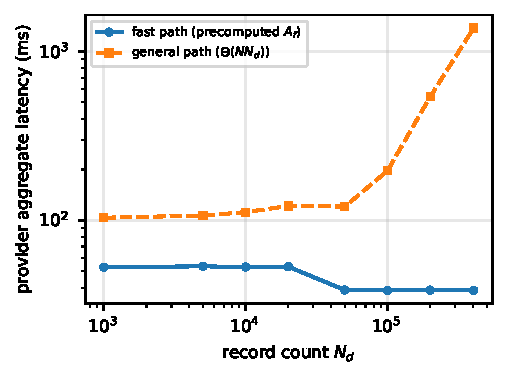
\includegraphics[width=0.72\linewidth]{figures/fig_aggregate_latency.pdf}
\caption{Aggregate latency, fast path against the single-round general path
(C++, two-ciphertext layout). The $x$-axis is $N_d$,
not $|S|$: cost no longer depends on the matched-set size. The fast path is
flat to $\pm0.5\%$ over a $405\times$ range.}
\label{fig:complat}
\end{figure}
\begin{table}[htbp]
\caption{Aggregate latency and storage, fast path against the single-round
general path, $N=11{,}580$, template \textsc{sum}, C++ prototype,
two-ciphertext layout. Medians of $11$ runs (fast) and $3$ (general).}
\label{tab:compute}
\centering
\footnotesize
\setlength{\tabcolsep}{3pt}
\renewcommand{\arraystretch}{1.2}
\begin{tabular*}{\tblwidth}{@{\extracolsep{\fill}}lcccc@{}}
\toprule
$N_d$ & Fast & General & $I'$ / provider & Downlink \\
      & (ms) & (ms)     & (GB)            & (B) \\
\midrule
$10^3$             & $38.8$ & $103.7$   & $0.09$  & $525{,}950$ \\
$5\times10^3$      & $39.0$ & $106.9$   & $0.46$  & $525{,}950$ \\
$10^4$             & $38.8$ & $111.9$   & $0.93$  & $525{,}950$ \\
$2\times10^4$      & $38.8$ & $121.7$   & $1.85$  & $525{,}950$ \\
$5\times10^4$      & $39.1$ & $120.7$   & $4.63$  & $525{,}950$ \\
$10^5$             & $39.2$ & $196.8$   & $9.26$  & $525{,}950$ \\
$2\times10^5$      & $39.1$ & $539.5$   & $18.53$ & $525{,}950$ \\
$4.05\times10^5$   & $38.8$ & $1{,}378.2$ & $37.54$ & $525{,}950$ \\
\bottomrule
\end{tabular*}
\end{table}

\subsection{Response packing, and what the trust split buys}
\label{sec:packresult}
Table~\ref{tab:packing} puts the two-ciphertext layout, the packed layout of
Section~\mref{sec:fast}, its compressed form and four-template responses
through the reference implementation at both corpora's tag domains, together
with baseline~(vi), a single server holding the same encrypted columns. All
rows come from one implementation on one machine and one thread, so they
compare with each other and not with the C++ figures. Byte counts are a
property of the parameters and of OpenFHE's serialisation, not of the
machine; the C++ prototype's $262{,}975$\,B per ciphertext against
$263{,}011$\,B here is a serialisation-version difference.

\begin{table}[htbp]
\caption{Fast path per provider: two-ciphertext against packed layouts, and a
single server on the same columns (baseline vi). Reference implementation,
one thread; medians of 21 runs. $k$ is the number of templates answered.}
\label{tab:packing}
\centering
\footnotesize
\setlength{\tabcolsep}{3pt}
\begin{tabular*}{\tblwidth}{@{\extracolsep{\fill}}lccc@{}}
\toprule
Layout & $k$ & Provider (ms) & Downlink (B) \\
\midrule
% --- generated from results/*.json by bench/make_tables.py ---
\multicolumn{4}{@{}l}{\emph{$N=11{,}580$ tags}} \\
Two ct (unpacked) & $1$ & $53.0$ & $526{,}022$ \\
Packed, 1 ct & $1$ & $23.5$ & $263{,}011$ \\
Packed + compressed & $1$ & $27.0$ & $132{,}081$ \\
$4\times$ two ct & $4$ & $194.9$ & $2{,}104{,}088$ \\
Packed, 1 ct & $4$ & $35.4$ & $263{,}011$ \\
Packed + compressed & $4$ & $32.7$ & $132{,}081$ \\
Single server (vi) & $1$ & $42.6$ & $263{,}211$ \\
\midrule
\multicolumn{4}{@{}l}{\emph{$N=35{,}162$ tags}} \\
Two ct (unpacked) & $1$ & $55.8$ & $526{,}022$ \\
Packed, 1 ct & $1$ & $31.4$ & $263{,}011$ \\
Packed + compressed & $1$ & $36.4$ & $132{,}081$ \\
$4\times$ two ct & $4$ & $245.6$ & $2{,}104{,}088$ \\
Packed, 1 ct & $4$ & $74.2$ & $263{,}011$ \\
Packed + compressed & $4$ & $92.3$ & $132{,}081$ \\
Single server (vi) & $1$ & $92.5$ & $263{,}211$ \\
\bottomrule
% ---
\end{tabular*}
\end{table}

\emph{Packing halves the provider's work and the downlink.} One rotate-and-sum
over half-rows replaces two over full rows: a single template falls from
$53.0$ to $23.5$\,ms at $N=11{,}580$ and from $55.8$ to $31.4$\,ms at
$N=35{,}162$, and the response from two ciphertexts to one, $263{,}011$\,B, or
$132{,}081$\,B compressed. Four templates in one compressed response cost
$32.7$\,ms and $132{,}081$\,B at $N=11{,}580$, against $194.9$\,ms and
$2{,}104{,}088$\,B for four two-ciphertext responses ($16\times$ less downlink).
At $N=35{,}162$ they need $35$ chunks instead of $12$, so the cost grows to
$74$--$92$\,ms while the response stays one ciphertext.

\emph{Against a single server, the trust split buys the client side.}
Baseline~(vi) needs no non-collusion assumption. Its server costs $42.6$ and
$92.5$\,ms at the two tag domains, $1.8$ and $2.9$ times one packed CR-SHE
provider ($23.5$ and $31.4$\,ms), because its contraction multiplies ciphertext
by ciphertext; its response is the same one ciphertext. The ratios compare one
provider with one server: two CR-SHE providers together spend $47.0$ and
$62.8$\,ms, so in total server work the trust split costs more than a single
server at the smaller tag domain and saves about a third at the larger. Its query is not (Table~\ref{tab:uplink}):
$789{,}033$ and $2{,}367{,}099$\,B of fresh ciphertexts against a $260$ or
$294$\,B DPF key per provider ($520$ and $588$\,B in total for two),
$3{,}035$ and $8{,}051$ times more uplink per provider, and $14.6$ and
$67.5$\,ms of client encryption against $0.54$ and $0.62$\,ms of key
generation. Query compression by ciphertext expansion \citep{angel2018pir}
would cut that uplink to one ciphertext for more server automorphisms; we did
not implement it.

\begin{table}[htbp]
\caption{Per-query uplink and client cost: CR-SHE's two-party key against the
single server's encrypted query. Reference implementation, one thread.}
\label{tab:uplink}
\centering
\footnotesize
\setlength{\tabcolsep}{3pt}
\begin{tabular*}{\tblwidth}{@{\extracolsep{\fill}}lcccc@{}}
\toprule
 & Key (B) & Enc.\ query (B) & Cts & Encrypt (ms) \\
\midrule
% --- generated from results/*.json by bench/make_tables.py ---
$N=11{,}580$ & $260$ & $789{,}033$ & $3$ & $14.6$ \\
$N=35{,}162$ & $294$ & $2{,}367{,}099$ & $9$ & $67.5$ \\
% ---
\bottomrule
\end{tabular*}
\end{table}

On retrieval a single server must bring every word of the packed
$N\times\lceil N_d/32\rceil$ index into contact with an encrypted one-hot
query, about $\lceil N\lceil N_d/32\rceil/\ell\rceil$ plaintext-ciphertext
products in a direct packed-selection formulation; query compression,
preprocessing or specialised PIR layouts may change that. At the measured
$0.092$\,ms per product this estimate is $81.6$\,ms at
$N_d=2\times10^4$ and $1.65$\,s at $N_d=405{,}184$, against $26.0$\,ms and
$1.10$\,s for CR-SHE's packed retrieval (Table~\ref{tab:packed}); across the
sweep the ratio is $1.5$--$3.1\times$ for that cost model, not against a
measured optimised single-server system, and the two figures come from separate
runs. The separation on every single-keyword path is therefore a small constant
factor in server work, set by a homomorphic slot operation ($11$\,ns here)
against a word operation, plus three orders of magnitude in uplink. That is the
honest case for the non-collusion assumption on these paths: it pays where the
client is thin or the link is metered, which is the IoT setting. On ranges
(Section~\mref{sec:rangeresult}) the gap is wider.

\subsection{The flexible path}
\label{sec:flexresult}
Table~\ref{tab:flex} reports the two rounds of a flexible query at
$N=11{,}580$ in the reference implementation, swept in decreasing $N_d$ to
control for warm-up. Round one, the retrieval, grows linearly with $N_d$ as
its $\Theta(NN_d)$ contraction predicts. Round two costs $20.1$--$35.6$\,ms
with no trend in $N_d$ over this range, because one to five packed products are
dwarfed by the twelve rotations of the row sum, and it returns one
$132{,}081$\,B ciphertext whatever the selection. Its uplink is a $16$\,B seed
to $n-1$ providers and $8N_d$\,B to one. Every flexible query in the reference implementation's tests, including
conjunctions, disjunctions and ad-hoc weights, decrypts to the plaintext ground
truth.

\begin{table}[htbp]
\caption{Flexible path, $N=11{,}580$, $n=2$, reference implementation, one
thread. Round-two uplink is the heavy provider's; the others receive 16\,B.}
\label{tab:flex}
\centering
\footnotesize
\setlength{\tabcolsep}{2pt}
\begin{tabular*}{\tblwidth}{@{\extracolsep{\fill}}lccccc@{}}
\toprule
$N_d$ & Round 1 & Round 2 & Up (B) & Down (B) & $I'$ \\
      & (ms)    & (ms)    &        &          & (GB) \\
\midrule
% --- generated from results/*.json by bench/make_tables.py ---
$1{,}000$ & $41.2$ & $20.1$ & $8{,}000$ & $132{,}081$ & $0.09$ \\
$5{,}000$ & $247.3$ & $35.6$ & $40{,}000$ & $132{,}081$ & $0.46$ \\
$10{,}000$ & $399.4$ & $21.9$ & $80{,}000$ & $132{,}081$ & $0.93$ \\
$20{,}000$ & $758.0$ & $26.4$ & $160{,}000$ & $132{,}081$ & $1.85$ \\
% ---
\bottomrule
\end{tabular*}
\end{table}

\subsection{Packed masked index}
\label{sec:packedresult}
Table~\ref{tab:packed} compares the masked index with one membership bit per
$\mathbb{Z}_p$ word against $32$ bits per word, at the primary corpus's tag
domain $N=11{,}580$, in the reference implementation. Packing divides the index
by exactly $32$ and makes retrieval $19$ to $27$ times faster at
$N_d=10^4$ and $2\times10^4$, where both layouts fit in this machine's memory.
At the full $405{,}184$ records the packed index is $1.17$\,GB, against
$37.5$\,GB unpacked (computed), and a retrieval takes $1.10$\,s and returns
$101{,}296$\,B per provider. Every retrieval returned exactly the posting list.

\begin{table}[htbp]
\caption{Masked index, unpacked against $32$ bits per word, $N=11{,}580$.
Reference implementation, one thread; retrieval per provider.}
\label{tab:packed}
\centering
\footnotesize
\begin{tabular*}{\tblwidth}{@{\extracolsep{\fill}}llccc@{}}
\toprule
$N_d$ & Layout & Index (GB) & Retrieval (ms) & Downlink (B) \\
\midrule
\inputtbl tables/packed.tex 
\bottomrule
\end{tabular*}
\end{table}

\subsection{Multi-cloud deployment}
\label{sec:wanresult}
With $n\in\{2,3,4\}$ separate provider processes and a client over TCP on one
host (Table~\ref{tab:wan}), provider compute is flat in $n$, at $34.82$,
$34.85$ and $35.48$\,ms, so the client waits on the slowest provider, not on
their sum. End-to-end latency rises from $44.1$ to $52.5$\,ms, all of it
transport of the $n$ responses; the client's combine, verify and decrypt cost
$1.37$--$1.63$\,ms. The transport covers loopback only: wide-area latency,
bandwidth variation, stragglers and recovery were not measured, so no fixed
cross-region increment can be inferred from these figures.

\begin{table}[htbp]
\caption{Single-host deployment over loopback, medians of 100 queries.
Transport excludes wide-area latency.}
\label{tab:wan}
\centering
\footnotesize
\setlength{\tabcolsep}{3pt}
\renewcommand{\arraystretch}{1.2}
\begin{tabular*}{\tblwidth}{@{\extracolsep{\fill}}lcccc@{}}
\toprule
$n$ & End-to-end & Provider & Transport & Client \\
    & (ms)       & (ms)     & (ms)      & (ms) \\
\midrule
$2$ & $44.12$ & $34.82$ & $8.30$  & $1.37$ \\
$3$ & $45.40$ & $34.85$ & $9.09$  & $1.52$ \\
$4$ & $52.53$ & $35.48$ & $15.48$ & $1.63$ \\
\bottomrule
\end{tabular*}
\end{table}

\subsection{Communication}
\label{sec:commresult}
At $N=11{,}580$ the two-party construction sends a $266$\,B key to each
provider, $532$\,B of uplink in total. The non-succinct $n$-party
instantiation used for $n>2$ sends $32$\,B to each of $n-1$ providers and
$92{,}656$\,B to one, so total uplink is $92{,}688$\,B at $n=2$,
$92{,}720$\,B at $n=3$ and $92{,}752$\,B at $n=4$. Tolerating more collusion
is therefore nearly free in this instantiation, but moving beyond two
providers at all costs a factor of $174$ in uplink over the succinct two-party
tree. A succinct
$(n{-}1)$-private instantiation would reduce the heavy key from $O(N\log p)$
to $O(2^{n/2}\sqrt{N}\lambda)$.


Downlink is $525{,}950$\,B per provider for an aggregate in the two-ciphertext
layout and $132{,}081$\,B packed and compressed, for up to four templates in
our configuration, and a fixed $\lceil N_d/32\rceil$ words for a retrieval,
which is $25{,}000$\,B at $N_d=10^5$ packed ($800{,}000$\,B unpacked), none
depending on $|S|$. A range query and a flexible round each return one
$132{,}081$\,B ciphertext.

\subsection{Setup, masking and ingest costs}
\label{sec:setupresult}
Unpacked, the mask costs a factor of $64$ in index storage over a plaintext
bitmap; packed, a factor of $2$. In the C++ prototype the unpacked masked index
at $N_d=10^5$ took $5.6$\,s to build, the fast-path column $A_f$ $1.2$--$12$\,ms
per template, occupying $2$ ciphertexts ($0.53$\,MB) whatever $N_d$, and a
complete provider bundle for the full corpus (context, evaluation keys, $pk$
and eight columns) was $12$\,MB and took $0.8$\,s to produce. Insertion into the hot
buffer ran at $4.5$--$14.1$ million records per second; a fast-path static-tier
rebuild cost $14.7$--$14.9$\,ms per template, $58.0\,\mu$s per insertion at
$B=256$ and $0.91\,\mu$s at $B=16{,}384$, while the buffer scan added
$98.8$--$100.0\%$ to a query. The range cube registered in
Section~\mref{sec:rangeresult} took $1.3$\,s (combined) and $9.8$\,s
(per-corner) to build and encrypt in the reference implementation.
\authorcheck{Re-measure the masked-index build with rejection sampling and
packing in C++.}


\subsection{Core scaling and throughput}
\label{sec:scaling}
In the C++ prototype a single fast-path query does not speed up with cores
($34.3$, $34.4$ and $38.4$\,ms at $1$, $8$ and $64$ threads), because the
homomorphic contraction dominates, but throughput does: $29.1$ queries/s with
one client, $56.9$ with two, $110.2$ with four, and a plateau of
$121.6$--$127.7$ from sixteen to sixty-four clients, with median latency rising
from $34.4$ to $516$\,ms; between four and sixteen clients throughput is within
$15\%$ of its maximum and median latency stays under $135$\,ms.

\subsection{Role-scoped access}
\label{sec:authresult}
Table~\ref{tab:roles} repeats the extraction attack of our earlier
measurement, in which a client sending raw additive shares of basis vectors
read every row of the masked index undetected (the C++ prototype recovered
$512$ of $512$ rows). The reference deployment has $512$ tags over three roles
of $4{,}096$ records each; the attacker holds role~$0$ and sends a raw share
vector for every row. With one mask key it recovers every row exactly, including
all $365{,}227$ membership bits that belong to the other two roles. With
role-scoped keys it recovers none of those bits and no row exactly; when it
applies its own key to the other roles' words, $6.06\%$ of them pass the width
check, against the $6.25\%$ expected of uniform words. Through the fast path the
same user obtained, for all $512$ tags, exactly the role-$0$ aggregate and in no
case the all-role one, and a flexible round asking for every record returned
the role-$0$ total. The price is storage: the aggregate columns, cube tables and
record column are held once per role, while the masked index, the largest
structure, is shared.

\begin{table}[htbp]
\caption{Index extraction by a role-$0$ user sending raw shares for all
$512$ rows; three roles of $4{,}096$ records. Reference implementation.}
\label{tab:roles}
\centering
\footnotesize
\begin{tabular*}{\tblwidth}{@{\extracolsep{\fill}}lccc@{}}
\toprule
Index & Rows exact & Other roles' bits & Other words \\
 & & recovered & pass width check \\
\midrule
\inputtbl tables/roles.tex 
\bottomrule
\end{tabular*}
\end{table}

\subsection{Second corpus: twelve sites and a larger tag domain}
\label{sec:secondcorpus}
The primary corpus has three devices, so its tag universe is dominated by time
buckets. The C++ prototype therefore repeated every experiment above on the
Beijing corpus, whose twelve sites give three times the tag domain
($N=35{,}162$, posting lengths median $12$, mean $131.5$, maximum $102{,}344$).
Missing readings get their own \texttt{:na} tag rather than falling into the
lowest band, since CO is missing in $4.92\%$ of records, and temperature is
shifted by $+50\,^\circ$C so that it stays non-negative. Every correctness
check passed unchanged, including a byte-identical $525{,}950$\,B downlink for
$|S|=0$ and $|S|=5{,}000$.

\emph{The fast path is unaffected by the larger tag domain.} It cost
$40.2$--$41.2$\,ms from $N_d=5\times10^3$ to $4.05\times10^5$
(Table~\ref{tab:beijing}), $5\%$ more than on the primary corpus for
$3.04\times$ the tags: the packed products grow from $2$ ciphertexts to $5$,
but the fixed rotate-and-sum, encryption and serialisation dominate. The first
point, $54.6$\,ms at $N_d=10^3$, carries the warm-up artefact of
Section~\ref{sec:aggresult}, since this sweep ran in increasing $N_d$.
\emph{The unpacked masked index is storage-bound.} The general path cost
$382.0$\,ms at $N_d=10^5$ against $196.8$\,ms on the primary corpus, and its
unpacked index grew to $28.13$\,GB; the harness refused the last two points,
which needed $56.26$ and $113.98$\,GB, against a $47.5$\,GB budget. Packing
(Section~\mref{sec:mask}) divides all of these by $32$, to $3.6$\,GB at
$N_d=4.05\times10^5$ (computed).

\begin{table}[htbp]
\caption{Second corpus ($N=35{,}162$, $N_d$ up to $420{,}370$): aggregate
latency and unpacked index size, template \textsc{sum}, C++ prototype,
two-ciphertext layout. Sweep in increasing $N_d$; ``n/a'' marks a point the
harness refused on its memory budget.}
\label{tab:beijing}
\centering
\footnotesize
\setlength{\tabcolsep}{3pt}
\begin{tabular*}{\tblwidth}{@{\extracolsep{\fill}}lcccc@{}}
\toprule
$N_d$ & Fast (ms) & General (ms) & $I'$ (GB) & Downlink (B) \\
\midrule
$10^3$             & $54.6$ & $106.3$ & $0.28$   & $525{,}950$ \\
$5\times10^3$      & $40.4$ & $86.9$  & $1.41$   & $525{,}950$ \\
$10^4$             & $40.2$ & $99.7$  & $2.81$   & $525{,}950$ \\
$2\times10^4$      & $40.5$ & $145.5$ & $5.63$   & $525{,}950$ \\
$5\times10^4$      & $40.7$ & $220.8$ & $14.06$  & $525{,}950$ \\
$10^5$             & $41.2$ & $382.0$ & $28.13$  & $525{,}950$ \\
$2\times10^5$      & $40.9$ & n/a     & $56.26$  & $525{,}950$ \\
$4.05\times10^5$   & $40.9$ & n/a     & $113.98$ & $525{,}950$ \\
\bottomrule
\end{tabular*}
\end{table}


\emph{The remaining measurements track the primary corpus.} Provider compute
in the single-host deployment was flat in $n$ ($38.67$, $37.65$ and
$38.47$\,ms for $n=2,3,4$), with end-to-end latency rising from $48.17$ to
$56.04$\,ms in transport alone. The DORY-style search-only baseline cost
$305.6$\,ms against $41.2$\,ms for the complete fast path, so the gap widens to
$7.4\times$ as $N$ grows; the homomorphic equality scan, $24.4$\,s, is
essentially unchanged, $592\times$ the fast path. Throughput plateaued at
$117$--$124$ queries/s; insertion into the hot buffer ran at $4.5$--$11.1$
million records per second; a fast-path static-tier rebuild cost
$28.7$--$29.1$\,ms, twice the primary corpus and linear in $N$; and building
the unpacked masked index at $N_d=10^5$ took $16.6$\,s against $5.6$\,s, while
$A_f$ stays $5$ ciphertexts ($1.3$\,MB). Selection latency and keys depend on
$N$ alone and were not re-measured: the two-party key is $300$\,B and the
$n$-party heavy key $8N+16=281{,}312$\,B, both computed.

\section*{S6. Withdrawn leakage figures from the C++ prototype}
\addcontentsline{toc}{section}{S6. Withdrawn leakage figures from the C++ prototype}

\emph{The C++ prototype's earlier figures are withdrawn.} An earlier run of the
attack in the C++ prototype reported higher unmasked recovery: $4.27\%$
overall on the primary corpus, $100\%$ in every non-temporal class of both
corpora, $3.80\%$ of one-minute windows and $0.31\%$ of hourly windows. Several
of these figures are not attainable by any attacker who sees only row
statistics. Rows with the same observed statistic are indistinguishable to such
an attacker, so whatever its strategy and auxiliary knowledge it expects at
most one correct assignment per distinct value: a class whose $n$ tags take
$v$ distinct lengths can lose at most $v/n$ of them, and the whole index at
most the number of distinct lengths over $N$. An hourly window of the second
corpus holds at most one record per site, so its length is one of at most
twelve values, whatever the corpus builder; in our build it takes seven, and at
most $0.020\%$ of the hourly windows can be re-identified, against the $0.31\%$
reported. The twelve sites share four lengths, so at most $33.3\%$ of them, not
$100\%$. On the primary corpus the one-minute windows take twenty lengths
(between $14$ and $43$ messages), a bound of $0.17\%$ against $3.80\%$, and the
whole index fifty-six, a bound of $0.484\%$ against $4.27\%$. The reference
attack meets these bounds exactly at $f=1$. The C++ attack must therefore have
used information beyond the lengths, most plausibly an order of tied
candidates that followed the true labels. The bounds are computed from the
per-tag lengths of our corpus build (\texttt{bench/leakage\_bounds.py}, which
also reproduces every unmasked, padded and volume-hiding rate from those
lengths and fails when a single tie is planted); only the twelve-value bound on
hourly windows holds for any build. We report the reference figures, which the
released code and data reproduce. The conclusion
is unchanged and is now measured against the standard defences: an unmasked
replicated index exposes the meaningful tag classes, power-of-two padding
still exposes many of them, and the masked index, like volume-hiding padding
but without its storage cost, leaves the attack at random guessing.
\authorcheck{If the C++ prototype is released, check its attack's
tie-breaking and compare its per-tag lengths with results/lengths\_*.csv.gz.}
\bibliographystyle{model1-num-names}
\bibliography{references}
\end{document}
